\documentclass{beamer}
\usepackage{beamerthemesplit}
\usepackage{wrapfig}
\usetheme{SPbGU}
\usepackage{pdfpages}
\usepackage{amsmath}
\usepackage{cmap} 
\usepackage[T2A]{fontenc} 
\usepackage[utf8]{inputenc}
\usepackage[english,russian]{babel}
\usepackage{indentfirst}
\usepackage{amsmath}
\usepackage{tikz}
\usepackage{multirow}
\usepackage[noend]{algpseudocode}
\usepackage{algorithm}
\usepackage{algorithmicx}
\usetikzlibrary{shapes,arrows}
\usepackage{fancyvrb}
\usepackage{tikz}
\usepackage{pgfplots}
\usetikzlibrary{calc}
\usetikzlibrary{shapes,arrows}
\usetikzlibrary{arrows,automata}
\usetikzlibrary{positioning}
\usepackage[labelformat=empty]{caption}
\usepackage[labelformat=empty]{subcaption}
\beamertemplatenavigationsymbolsempty
\usepackage{multirow}
\usepackage{verbatim}
\usepackage{array}
\usepackage{graphicx}
\usepackage{multirow} 
\usepackage{fancyvrb}
\usepackage[misc,geometry]{ifsym} 
\newcolumntype{P}[1]{>{\centering\arraybackslash}p{#1}}


\newcommand{\tikzmark}[1]{\tikz[overlay,remember picture] \node (#1) {};}
\def\Put(#1,#2)#3{\leavevmode\makebox(0,0){\put(#1,#2){#3}}}

\newcommand{\ltz}{$< 1$}
\tikzset{
    state/.style={
           rectangle,
           rounded corners,
           draw=black, very thick,
           minimum height=2em,
           inner sep=4pt,
           text centered,
           },
}

\newtheorem{rutheorem}{Теорема}
\newtheorem{task}{All-paths CFPQ problem and reachability CFPQ problem }
\newtheorem{ruproof}{Доказательство}
\newtheorem{rudefinition}{Определение}
\newtheorem{rulemma}{Лемма}


\title[GLL for Graph]{Implementation and experimental study of GLL algorithm with Neo4j graph database}
\institute[]{
JetBrains Research, Programming Languages and Tools Lab \\
St Petersburg State University }

\author[Vlada Pogozhelskaya]{Vlada Pogozhelskaya}


\date{December 17, 2021}
\begin{document}
{
\begin{frame}[fragile]
  \begin{tabular}{p{2.0cm} p{7.5cm} p{1cm}}
   \begin{center}
      
\includegraphics[height=1.5cm]{pics/jetbrainsResearch.pdf}
    \end{center}
    &
    \begin{center}
      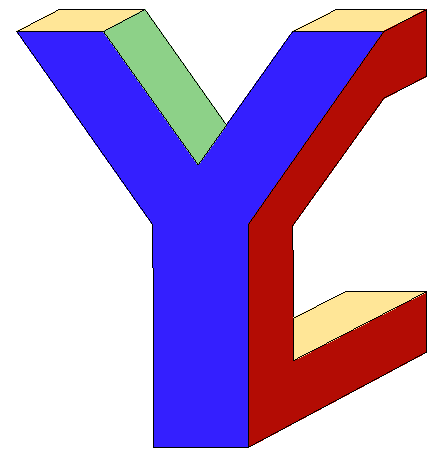
\includegraphics[height=1.5cm]{pics/YC_logo.pdf}
    \end{center}
    &
    \begin{center}
      
\includegraphics[height=1.5cm]{pics/SPbGU_Logo.png}
    \end{center}
  \end{tabular}
  \titlepage
\end{frame}
}
\begin{frame}[fragile]
  \transwipe[direction=90]
  \frametitle{Introduction}
  \begin{itemize}
      \item Graph data model
      \begin{itemize}
        \item Basic entities --- graph vertices
        \item Relationships between entities are stored in the graph model itself
      \end{itemize}
    \item Graph databases
\begin{itemize}
    \item The most popular is Neo4j
    \item Only regular queries are partially supported
\end{itemize} 
\item Context-free constraints
\begin{itemize}
    \item Strictly more expressive than the regular one
    \item Widely used in bioinformatics, RDF file analysis, static code analysis
\end{itemize}
\end{itemize}
\end{frame}

\begin{frame}[fragile]
  \transwipe[direction=90]
  \frametitle{Context-free path querying problems}
   \begin{task}
  Let be:
     \begin{itemize}
    \item Context-free grammar $\mathbb{G}  = \langle N, \Sigma, P, S \rangle$
     \item Directed graph $ \mathbb{D} = \langle V, E, T \rangle$
     \item Set of start vertices $V_S \subseteq V$  and set of final vertices \mbox{$V_F \subseteq V$}
\end{itemize} 
\textbf{All-paths problem}:
\begin{itemize}
    \item Find all paths $\pi = (e_0, e_1, \cdots, e_{n - 1}, e_n), ~ e_k = (v_{k - 1}, t_k, v_k)$ in graph $ \mathbb{D}$, such as $l(\pi) = t_1t_2 \cdots t_n \in L(\mathbb{G})$ and $v_0 \in V_S, ~v_n \in V_F$
\end{itemize}
\textbf{Reachability problem}:
\begin{itemize}
    \item Find all pairs $\{(v_i, v_j ) ~|~ \exists ~l(\pi) \in L(\mathbb{G})$ и $v_0 \in V_S, ~v_n \in V_F\}$
\end{itemize}
 \end{task}
\end{frame}

\begin{frame}[fragile]
  \transwipe[direction=90]
  \frametitle{Motivation}
  \begin{itemize}
        \item The problem of poor performance of CFPQ algorithms was formulated by Jochem Kuijpers as a result of an attempt to extend Neo4j
      \item Later, the matrix-based CFPQ algorithm showed high performance on real-world data
  \end{itemize}
\end{frame}

\begin{frame}
  \transwipe[direction=90]
  \frametitle{Overview}
  \textbf{Generalized LL algorithm (GLL)}
\begin{itemize}
    \item Supports the entire class of context-free languages
    \item To reconstruct the paths the Shared Packed Parse Forest (SPPF) is supported
\end{itemize}
\textbf{Proposed solution}\\
  \begin{itemize}
    \item Based on GLL algorithm implementation in Iguana\footnote{ Repository of Iguana project: \url{https://github.com/iguana-parser/iguana}} project
    \item The ability to return as a result both a set of pairs of reachable vertices and the constructed SPPF 
    \item Neo4j graph database is used as a graph storage
    \item The solution was integrated with Neo4j using Native Java API
  \end{itemize}
  \end{frame}
  
  \begin{frame}
\transwipe[direction=90]
 \frametitle{Experimental study of proposed solution}
 \textbf{Data}
 \begin{itemize}
     \item \textbf{RDF Graphs}
     \begin{itemize}
         \item \textit{Grammars}
  \begin{align}
\begin{split}
\label{eqn:g_1}
S \to & \overline{\textit{subClassOf}} \ \ S \ \textit{subClassOf} \mid \overline{\textit{type}} \ \ S \ \textit{type}\\   & \mid \overline{\textit{subClassOf}} \ \ \textit{subClassOf} \mid \overline{\textit{type}} \ \textit{type}
\end{split}
\end{align}
\begin{align}
\label{eqn:g_2}
S \to \overline{\textit{subClassOf}} \ \ S \ \textit{subClassOf} \mid \textit{subClassOf}
\end{align}
\begin{align}
\begin{split}
\label{eqn:geo}
S \to & \textit{broaderTransitive} \ \  S \ \overline{\textit{broaderTransitive}} \\
      & \mid \textit{broaderTransitive} \ \  \overline{\textit{broaderTransitive}}
\end{split}
\end{align}
     \end{itemize}
     \item \textbf{Program analysis graphs}
     \begin{itemize}
         \item 
         \textit{Grammar}
         \begin{align}
\begin{split}
\label{eqn:points_to}
M & \to \overline{d} \ V \ d \\
V & \to (M? \ \overline{a})^* \ M? \ (a \ M?)^* 
\end{split}
\end{align}
     \end{itemize}
 \end{itemize}
 \end{frame}
 
 \begin{frame}
\transwipe[direction=90]
 \frametitle{All pairs results}
  \begin{figure}[H]
\centering
\alt<2>{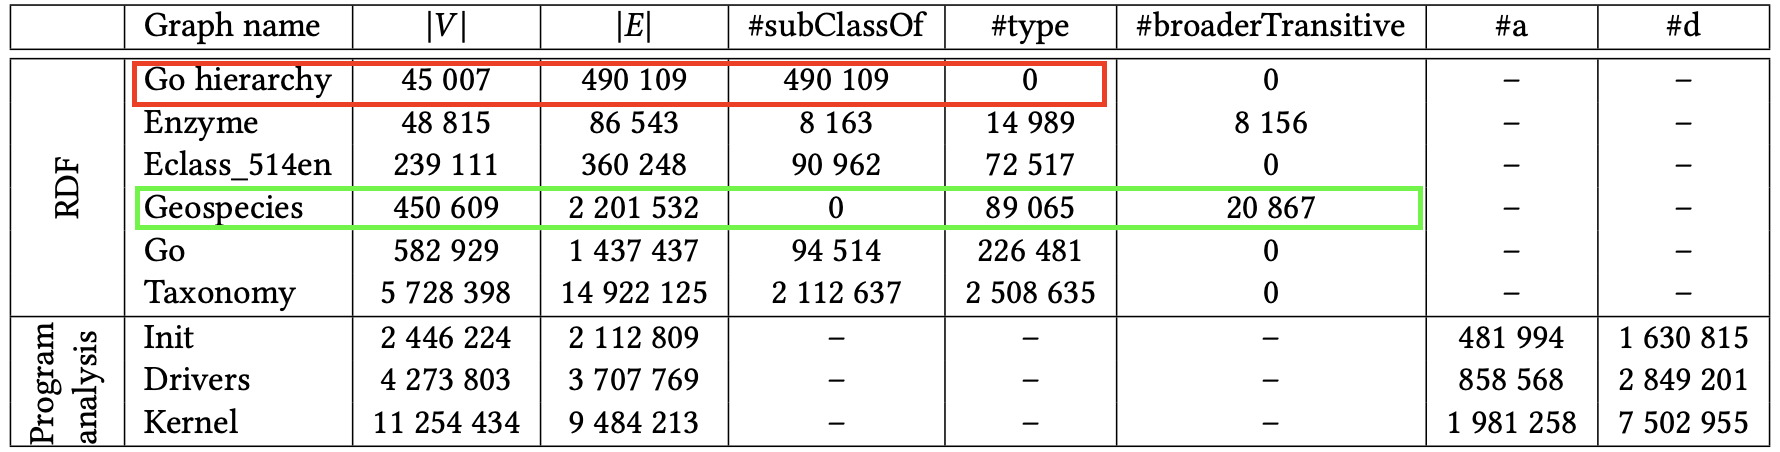
\includegraphics[width=0.9\textwidth]{Pogozhelskaya/pics/nums_go.png}}{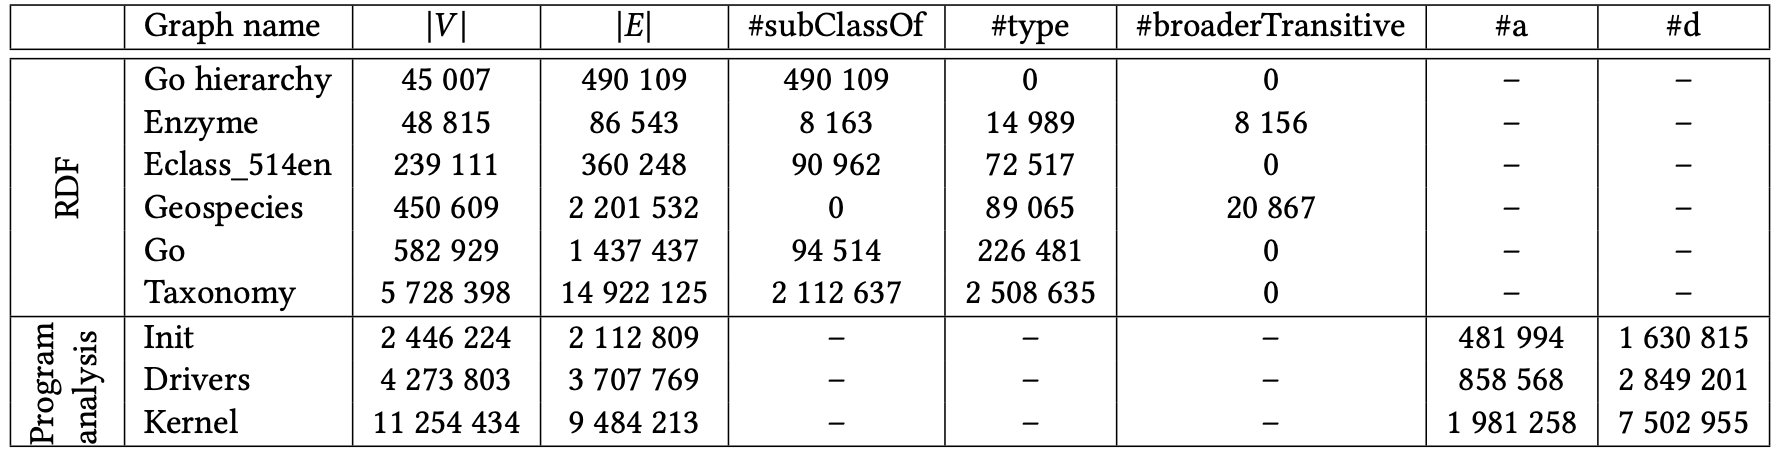
\includegraphics[width=0.9\textwidth]{Pogozhelskaya/pics/nums.png}}
\label{fig:nums}
\end{figure}

 \begin{figure}[H]
\centering
\alt<2>{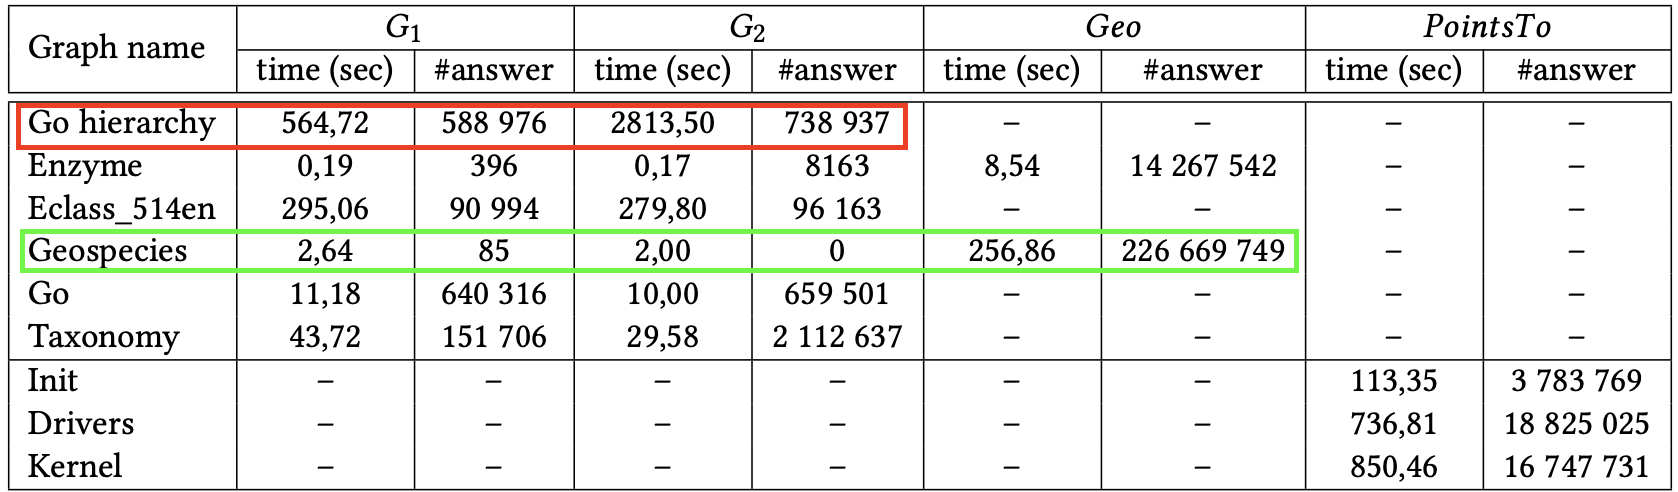
\includegraphics[width=0.9\textwidth]{Pogozhelskaya/pics/res_go.png}}{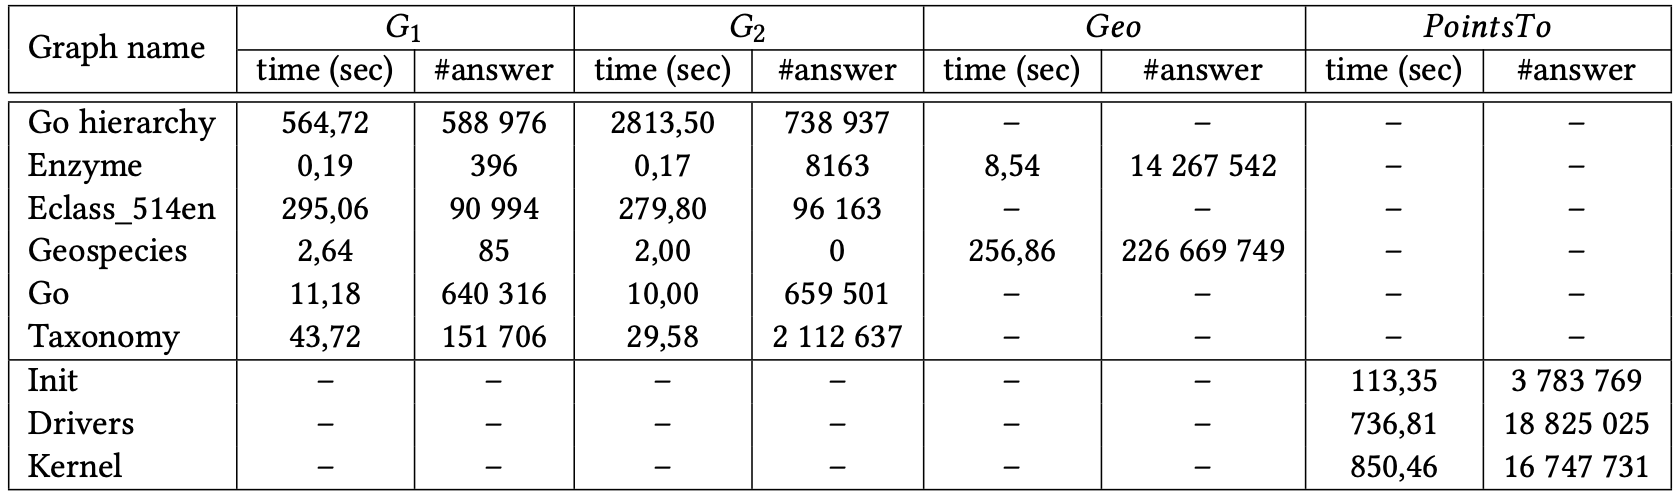
\includegraphics[width=0.9\textwidth]{Pogozhelskaya/pics/res.png}}
\label{fig:arch}
\end{figure}
\end{frame}

 \begin{frame}
\transwipe[direction=90]
 \frametitle{Multiple-source results}
 \begin{figure}[H]
\centering
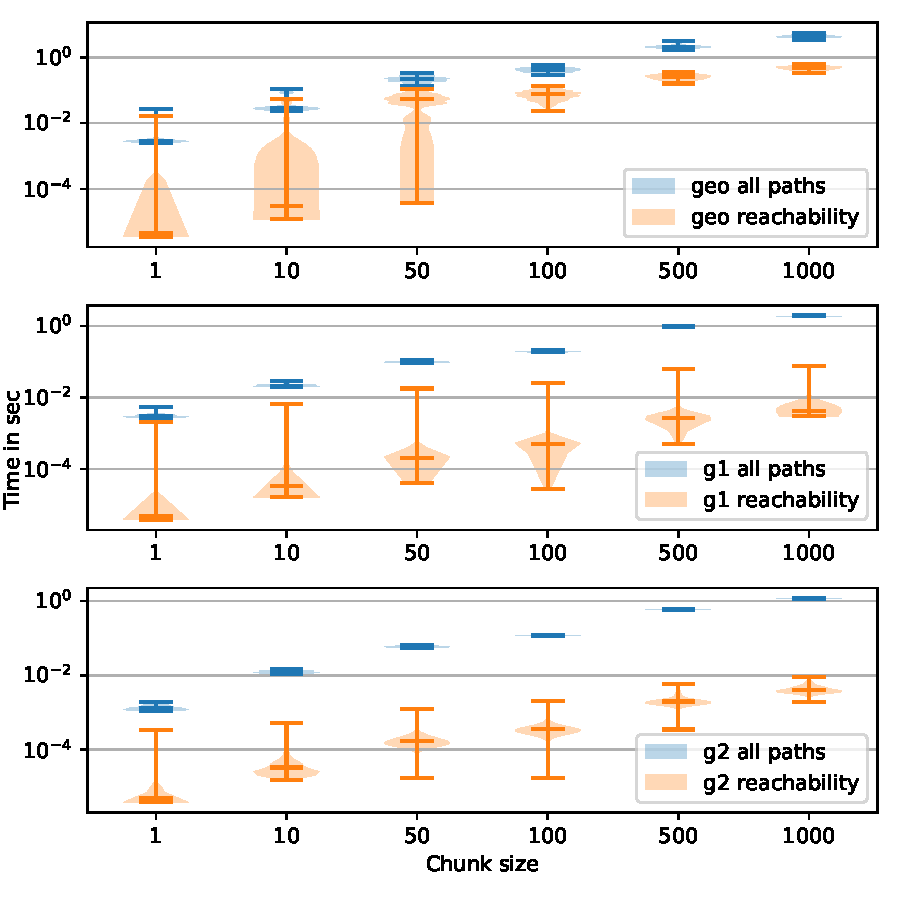
\includegraphics[width=0.7\textwidth,height=7.5cm]{Pogozhelskaya/pics/geospecies_chunks.pdf}
\label{fig:arch}
\end{figure}
\end{frame}

\begin{frame}
\transwipe[direction=90]
\frametitle{Results}
\begin{itemize}
    \item Not only the matrix-based algorithm is applicable to real-world data
    \item Results are submitted to EDBT conference
    \item Discussion with Neo4j team about a deeper algorithm integration is in progress
    \item The main direction of further research is to find a way to effectively parallelize the GLL algorithm
\end{itemize}
\end{frame}


\end{document}